\documentclass[10pt,leqno]{amsart}
\usepackage{graphicx}
\usepackage{indentfirst,csquotes}
\usepackage{booktabs}
\usepackage{amsmath,amssymb,amsthm}
\usepackage{xcolor,hyperref,paralist,titlesec,fancyhdr,etoolbox}
\usepackage[numbers,sort&compress]{natbib}

\topmargin= .5cm
\textheight= 20cm
\textwidth= 32cc
\baselineskip=16pt
\evensidemargin= .9cm
\oddsidemargin= .9cm

\hypersetup{colorlinks=true, linkcolor=black, filecolor=black, urlcolor=blue, citecolor=blue}

\titleformat{\section}[display]{\normalfont\huge\bfseries\centering}{\centering\chaptertitlename\thechapter}{10pt}{\Large}
\titlespacing*{\section}{0pt}{0ex}{0ex}

\newtheorem{theorem}{Theorem}[]
\newtheorem{definition}[theorem]{Definition}
\newtheorem{example}[theorem]{Example}
\newtheorem{lemma}[theorem]{Lemma}
\newtheorem{proposition}[theorem]{Proposition}
\newtheorem{corollary}[theorem]{Corollary}
\newtheorem{conjecture}[theorem]{Conjecture}

\begin{document}

\title{Eureka-from-CLIP: Parameter-Efficient BERT Adaptation for Zero-Shot Text-to-Video Retrieval}

\author{Siyuan Zhang$^{*\dagger}$\quad Yadi Cheng$^{\dagger}$\\[4pt]
  \small Zhejiang University of Technology\\
  \small\texttt{\{zhangsiyuan,chengyadi\}@zjut.edu.cn}}


\maketitle

\let\thefootnote\relax
\footnotetext{$^{*}$Corresponding author.}
\footnotetext{$^{\dagger}$Equal contribution.}

\begin{abstract}
We present Eureka-from-CLIP, a framework that replaces CLIP's fixed text encoder with a lightweight BERT-based encoder for zero-shot text-to-video retrieval under tight resource constraints. Through parameter-efficient cross-modal alignment, we first adapt BERT to CLIP's frozen visual space on COCO captions with only 1.35M trainable LoRA \citep{hu2022lora} parameters, outperforming CLIP's native text encoder on Flickr30k \citep{plummer2015flickr30k} text-to-image retrieval (60.48\% vs.~57.90\%). We then domain-adapt to video via Stack LoRA: freezing the COCO-trained adapter and adding a smaller rank-2 stack (0.63M trainable parameters) on MSR-VTT. The resulting model outperforms CLIP's zero-shot video retrieval on MSVD (28.13\% vs.~27.01\% t2i R@1) while using a tiny fraction of the training budget for adaptation. Our asymmetric queue design compensates for the small batch size mandated by limited GPU memory by masking stale text embeddings while retaining the fresh image queue. This work provides a practical recipe for replacing CLIP's text encoder with arbitrary BERT variants under limited compute, with direct applicability to both image and video retrieval, and naturally extends to multilingual settings via BERT's multilingual variants.
\end{abstract}

\bigskip

\section{Introduction}

CLIP \citep{radford2021clip} has become a de facto backbone for zero-shot text-to-video retrieval: per-frame CLIP vision embeddings are mean-pooled into a video representation and compared against CLIP's text encoder for retrieval \citep{luo2022clip4clip}. Despite its effectiveness, CLIP's text encoder is a fixed component --- it cannot be easily replaced or extended to support multilingual queries, domain-specific vocabulary, or more capable language models. Replacing it with an alternative encoder such as BERT \citep{devlin2019bert} would unlock these capabilities, but requires re-aligning the new encoder to CLIP's frozen visual space, a process that is non-trivial under limited computational resources.

In this work, we address the problem of replacing CLIP's text encoder with BERT for zero-shot text-to-video retrieval on a single 8\,GB GPU. Our key insight is that the alignment can be decomposed into two lightweight stages: first, adapt BERT to CLIP's visual space on image data where abundant captions exist; second, efficiently transfer the aligned encoder to the video domain with minimal forgetting of the original alignment.

We adopt LoRA \citep{hu2022lora} for parameter-efficient adaptation, training only low-rank adapters inserted into BERT's Transformer layers while keeping all pre-trained weights frozen. To compensate for the small batch size enforced by limited GPU memory, we employ a queue-based contrastive objective \citep{he2020moco}. However, training only the text encoder creates a staleness problem: as the text encoder evolves, text embeddings stored in the queue become outdated. We address this with an asymmetric queue design that masks stale text embeddings while retaining the full image queue, which stays perpetually fresh because it comes from a frozen CLIP vision encoder.

Our two-stage approach proceeds as follows. In Stage~1 (image alignment), we train BERT with LoRA (r=8, 1.35M trainable parameters) on COCO captions to align with CLIP's frozen image embeddings, achieving 60.48\% text-to-image R@1 on Flickr30k --- surpassing CLIP's native text encoder (57.90\%). In Stage~2 (video domain adaptation), we adapt the COCO-aligned BERT to MSR-VTT video captions via Stack LoRA: we freeze the COCO-trained adapter via weight merging and add a smaller rank-2 adapter (0.63M trainable parameters) that learns only the domain shift. The resulting model achieves 28.13\% t2i R@1 on MSVD zero-shot video retrieval, exceeding CLIP's baseline of 27.01\% in the same evaluation setup.

Our contributions are:

\begin{enumerate}
    \item We introduce an asymmetric queue design that masks stale text embeddings while retaining the fresh image queue, enabling effective small-batch contrastive learning when only the text encoder is trained.
    \item We propose Stack LoRA, a two-stage parameter-efficient strategy that freezes a pre-trained adapter via weight merging and stacks a smaller adapter for domain transfer, reducing forgetting while using fewer trainable parameters.
    \item We demonstrate that a BERT encoder aligned to CLIP's visual space via lightweight LoRA adaptation exceeds CLIP's native text encoder on both image (Flickr30k, 60.48\% t2i R@1) and video (MSVD, 28.13\% t2i R@1) zero-shot retrieval, using only 0.63--1.35M trainable parameters on a single 8\,GB GPU.
\end{enumerate}

Furthermore, because our framework uses BERT as the text encoder, it naturally supports multilingual retrieval by substituting multilingual BERT variants. We show that a multilingual BERT trained solely on English captions achieves non-trivial zero-shot Chinese retrieval (27.22\% t2i R@1 on Flickr30k), demonstrating cross-lingual generalization without any multilingual training data.

\section{Related Work}

\subsection{Text-to-Video Retrieval}

Transferring image-text models to video retrieval has been an active direction. CLIP4Clip \citep{luo2022clip4clip} provides the first systematic study of adapting CLIP to video-text retrieval, exploring multiple similarity computation mechanisms including mean pooling, sequential Transformers, and cross-modal attention. A key finding is that on small-to-medium datasets such as MSR-VTT and MSVD, the simple parameter-free mean pooling of frame embeddings outperforms more complex temporal architectures, because introducing additional trainable parameters on limited data can hurt the pretrained representations. This directly motivates our use of mean pooling over frame embeddings as the video representation. ClipBERT \citep{lei2021clipbert} proposes random sparse sampling (as few as 1--2 clips per video) during training, demonstrating that sparse sampling enables end-to-end learning without dense video features. Frozen in Time \citep{bain2021frozen} introduces a curriculum learning schedule that transitions from individual frames to temporal context, and proposes the WebVid-2M dataset for video-text pre-training. More recent works such as X-Pool \citep{gorti2022xpool} use cross-modal attention for frame aggregation, TS2-Net \citep{liu2022ts2net} introduces token shift and selection mechanisms for fine-grained spatio-temporal modeling, and VoP \citep{huang2023vop} adopts prompt tuning with only 0.1\% trainable parameters for efficient video-text adaptation.

\subsection{Replacing CLIP's Text Encoder}

LiT \citep{zhai2022lit} (Locked-image Tuning) freezes a pre-trained image encoder and trains only the text encoder to align with it via contrastive learning, demonstrating that locking the image encoder consistently outperforms fine-tuning it. This directly motivates our decision to freeze CLIP's vision encoder. While LiT treats the full text tower as trainable, we explore a more parameter-efficient alternative: we freeze BERT entirely and inject only low-rank adapters, achieving competitive alignment with substantially fewer trainable parameters. AltCLIP \citep{chen2022altclip} replaces CLIP's text encoder with XLM-R for multilingual capabilities, using a two-stage distillation-then-contrastive training process. Chinese CLIP \citep{yang2022chinese} builds a Chinese-specific vision-language model from scratch. Our work differs in that we focus on lightweight adaptation of BERT to CLIP's existing embedding space, requiring only a fraction of the training data and compute while supporting both image and video retrieval.

\subsection{Parameter-Efficient Cross-Modal Adaptation}

LoRA \citep{hu2022lora} proposes low-rank decomposition matrices inserted into pre-trained Transformer layers, dramatically reducing trainable parameters. This has been extended to video-language tasks: VoP \citep{huang2023vop} introduces prompt tuning on both text and video encoders with only 0.1\% trainable parameters. RAP \citep{cao2024acl} proposes sparse-and-correlated adapters with low-rank modulation for video-text fine-tuning. Our work introduces Stack LoRA, which extends the single-adapter paradigm by freezing a pre-trained LoRA via weight merging and stacking a smaller adapter for domain transfer --- enabling parameter-efficient video domain adaptation without forgetting the original alignment.

\subsection{Queue-based Contrastive Learning}

MoCo \citep{he2020moco} introduces a queue-based dictionary for contrastive learning, decoupling dictionary size from batch size. This is especially valuable in resource-constrained settings. However, when only the text encoder is trained and evolves over time, queued text embeddings become stale. Our asymmetric queue design directly addresses this: we completely mask the text queue for the image-to-text direction to avoid stale gradient contamination, while retaining the full image queue for text-to-image learning. Because the CLIP vision encoder is frozen, image embeddings in the queue remain perpetually fresh, making this asymmetry a natural fit for our setup.

\section{Method}

\subsection{Two-Stage Training Pipeline}

Our framework replaces CLIP's text encoder with a BERT encoder followed by a lightweight projection head. We decompose the training into two stages:

\textbf{Stage~1 -- Cross-modal alignment (image):} We train on COCO captions (113k images, 567k captions) to align BERT's output space with CLIP's frozen visual embedding space. This stage establishes a strong cross-modal initialization: after 30 epochs on a single 8\,GB GPU, the BERT encoder \emph{alone} outperforms CLIP's native text encoder on Flickr30k zero-shot retrieval (60.48\% vs.\ 57.90\%), using only 1.35M trainable LoRA parameters.

\textbf{Stage~2 -- Video domain adaptation:} We adapt the COCO-aligned BERT to MSR-VTT video captions. Because the text distribution shifts from COCO's concise captions to MSR-VTT's more descriptive video narrations, further training risks forgetting the cross-modal alignment established in Stage~1. To mitigate this, we introduce \textbf{Stack LoRA}: we first merge the COCO-trained LoRA adapter (r=8) into BERT's weights via \texttt{merge\_and\_unload()}, then add a new trainable LoRA adapter with a smaller rank (r=2) on top. The merged r=8 adapter is frozen in the base weights, while only the smaller r=2 adapter (0.63M trainable parameters) learns the video domain shift. This preserves the general cross-modal alignment while efficiently adapting to the target domain.

Because the CLIP vision encoder is frozen throughout both stages, video embeddings are precomputed once offline and mean-pooled from per-frame keyframe features, following the standard practice established by CLIP4Clip \citep{luo2022clip4clip}. The frozen encoder also guarantees that image/video embeddings in the contrastive queue never become stale.

\begin{figure}[h]
\centering
\includegraphics[width=\textwidth]{figures/figure1.png}
\caption{Training pipeline of Eureka-from-CLIP. Frozen CLIP vision encoder precomputes video frame or image embeddings (never stale). Trainable BERT text encoder with LoRA produces text embeddings. The image queue supplies abundant negatives for t2i learning, while the stale text queue is masked out.}
\label{fig:pipeline}
\end{figure}

\subsection{Model Architecture}

The model consists of three components:

\textbf{Frozen CLIP Vision Encoder.} We use OpenAI's ViT-B/32 as the frozen vision encoder. All images are encoded once offline, producing 512-dimensional L2-normalized embeddings.

\textbf{BERT Text Encoder.} We use BERT-base (uncased) as the text encoder backbone. For each input caption, BERT's [CLS] token representation is extracted from the final layer.

\textbf{Projection Head.} A linear projection maps the 768-dimensional BERT [CLS] embedding to the 512-dimensional shared space, followed by L2 normalization.

\textbf{LoRA Adapters (Stage~1).} We insert LoRA \citep{hu2022lora} adapters with rank $r=8$ and $\alpha=16$ into BERT's query, key, value, and output projection layers. The original BERT weights remain frozen; only the LoRA parameters and projection head are trainable. This results in 1.35M trainable parameters out of 110.8M total.

\textbf{Stack LoRA (Stage~2).} For video domain adaptation, we first merge the trained r=8 adapter into BERT's weights using PEFT's \texttt{merge\_and\_unload()}, which computes $W' = W + \frac{\alpha}{r}BA$ for each target layer and returns a plain model. We then insert a new LoRA adapter with rank $r=2$ and $\alpha=4$. The merged r=8 weights remain frozen in the base model; only the r=2 adapter (0.63M trainable parameters) is trained. This stacked design enables efficient domain transfer with minimal forgetting of the original cross-modal alignment.

\subsection{Loss Design}

We employ a weighted asymmetric InfoNCE loss \citep{oord2018representation} formulated as:

\begin{equation}
\mathcal{L} = (1 - \alpha) \cdot \text{CE}(\mathbf{S}_{i2t} \cdot \tau, \mathbf{y}) + \alpha \cdot \text{CE}(\mathbf{S}_{t2i} \cdot \tau, \mathbf{y}),
\label{eq:asymmetric_loss}
\end{equation}

where $\mathbf{S}_{i2t} = \mathbf{I} \mathbf{T}^{\top}$ is the image-to-text similarity matrix, $\mathbf{S}_{t2i} = \mathbf{T} \mathbf{I}^{\top}$ is the text-to-image similarity matrix, $\tau = \exp(\gamma)$ is a learnable temperature parameter initialized to $1/0.07$, $\mathbf{y}$ is the set of diagonal labels (positive pairs), $\text{CE}$ denotes cross-entropy, and $\alpha$ is the t2i weight.

We set $\alpha = 0.75$, giving 3$\times$ more weight to the text-to-image direction. This design choice is motivated by real-world usage: in text-to-image retrieval, the user provides a text query and the system retrieves relevant images or scenes, making text-to-image recall the more important metric.

\subsection{Queue Design with Text Staleness Masking}

Contrastive learning benefits from a large number of negative samples. Following MoCo \citep{he2020moco}, we maintain a FIFO queue of past (image, text) embedding pairs. However, a key challenge arises: the text encoder is being trained, so text embeddings in the queue were produced by earlier, less capable versions of the model. These ``stale'' text embeddings, if used as negatives for the image-to-text direction, can provide misleading gradient signals.

Our core insight is that this staleness is direction-dependent, and the asymmetry aligns perfectly with our task objective:

\begin{itemize}
    \item \textbf{Image-to-text (i2t):} The text queue is stale (text encoder evolves). We completely mask the text queue for this direction, using only in-batch negatives. This effectively means $\mathbf{S}_{i2t}$ in Eq.~\ref{eq:asymmetric_loss} is computed as $\mathbf{I}_{\text{batch}} \mathbf{T}_{\text{batch}}^{\top}$ without queue entries. Since t2i is our primary concern, sacrificing i2t queue negatives is an acceptable trade-off.
    \item \textbf{Text-to-image (t2i):} The image queue is \emph{not} stale because image embeddings come from a frozen CLIP encoder. We therefore retain the full image queue for this direction, computing $\mathbf{S}_{t2i} = \mathbf{T}_{\text{batch}} [\mathbf{I}_{\text{batch}}; \mathbf{I}_{\text{queue}}]^{\top}$. The fresh image queue provides a large and consistent set of negatives that directly boosts t2i performance.
\end{itemize}

This asymmetric queue design is illustrated in Table~\ref{tab:queue}. Importantly, the choice of which encoder to train and which queue side to keep is not arbitrary. If we had chosen to train the vision encoder while freezing the text encoder, the image embeddings would become stale and the text queue would remain fresh; the queue would then boost i2t instead of t2i --- the opposite of what we need. Our configuration (training text encoder, retaining the image queue) therefore creates a natural alignment between the training objective and the architectural design: the frozen CLIP guarantees a fresh image queue, and the fresh image queue guarantees strong t2i learning. By masking stale text embeddings, we further avoid damaging the i2t gradient, which is doubly beneficial since t2i already receives higher weight in the loss ($\alpha = 0.75$).

\begin{table}[h]
\centering
\caption{Asymmetric queue design for text-staleness-aware contrastive learning.}
\label{tab:queue}
\begin{tabular}{c|c}
\hline
\textbf{i2t direction} & \textbf{t2i direction} \\
In-batch negatives only & In-batch + queue negatives \\
\hline
$\mathbf{I}_{\text{batch}} \mathbf{T}_{\text{batch}}^{\top}$ & $\mathbf{T}_{\text{batch}} [\mathbf{I}_{\text{batch}}; \mathbf{I}_{\text{queue}}]^{\top}$ \\
No queue (avoid stale texts) & Image queue (no staleness) \\
\hline
\end{tabular}
\end{table}

We additionally apply false-negative masking: queue entries sharing the same image ID as a batch item are masked out (set to $-\infty$) in the similarity matrix, preventing them from being treated as negatives.

\subsection{Training Details}

\textbf{Stage~1 (image alignment)} We train on COCO train2017 captions (113k images, 567k captions) using a single GeForce RTX 4060 Laptop GPU with 8 GB VRAM:
\begin{itemize}
    \item Batch size: 128 (maximum that fits in 8 GB VRAM with BERT-base + LoRA)
    \item Optimizer: AdamW with learning rate $3\times 10^{-4}$, weight decay 0.01
    \item Scheduler: Linear warmup (34,536 steps) followed by cosine decay to zero
    \item Epochs: 30
    \item Mixed precision (AMP) for computational efficiency
    \item Queue size: 49,152
    \item LoRA rank: 8, alpha: 16, dropout: 0.1
\end{itemize}
The queue is updated after loss computation to prevent current-batch items from acting as their own negatives. Precomputed CLIP image embeddings avoid redundant vision forward passes. The entire Stage~1 training completes in approximately 12 hours.

\textbf{Stage~2 (video domain adaptation)} We train on MSR-VTT training captions (9k video clips, 180k caption-clip pairs) with the same GPU:
\begin{itemize}
    \item Batch size: 128
    \item Optimizer: AdamW with learning rate $1\times 10^{-5}$ (lower to preserve alignment)
    \item Scheduler: Linear warmup (4,000 steps) followed by cosine decay
    \item Epochs: 30
    \item Mixed precision (AMP)
    \item Queue size: 49,152
    \item Stack LoRA rank: 2, alpha: 4, dropout: 0.1
\end{itemize}
We evaluate on MSVD (1,970 videos, zero-shot) and Flickr30k (1K images) at the end of each epoch. For video, CLIP per-frame keyframe embeddings are mean-pooled into a video-level representation.

\section{Experiments}

\subsection{Evaluation Setup}

We evaluate on two benchmarks spanning video and image retrieval:

\textbf{MSVD} \citep{chen2011collecting} is a video retrieval benchmark containing 1,970 videos from YouTube, each annotated with approximately 20 human-written captions. Following the zero-shot protocol, we evaluate on the standard 670-video test split without any training on MSVD. Video representations are obtained by mean pooling 12 uniformly sampled CLIP per-frame keyframe embeddings, following the simple yet effective pooling strategy validated by CLIP4Clip \citep{luo2022clip4clip}.

\textbf{Flickr30k} \citep{plummer2015flickr30k} is an image retrieval benchmark with 31,783 images, each with 5 captions. We use the standard 1,000-image test set for zero-shot evaluation.

For the CLIP baseline on both benchmarks, we use the official OpenAI ViT-B/32 model. On the visual side, this is the same frozen encoder used during our BERT training. On the text side, we use CLIP's native Transformer text encoder.

\subsection{Main Results}

Table~\ref{tab:video_results} presents the main results on MSVD video retrieval. Our two-stage approach achieves competitive performance:

\begin{table}[h]
\centering
\caption{Zero-shot text-to-video retrieval results on MSVD. All methods use the same frozen CLIP ViT-B/32 vision encoder with mean-pooled frame embeddings.}
\label{tab:video_results}
\begin{tabular}{lcccccc}
\toprule
Method & \multicolumn{3}{c}{t2i} & \multicolumn{3}{c}{i2t} \\
\cmidrule(lr){2-4} \cmidrule(lr){5-7}
 & R@1 & R@5 & R@10 & R@1 & R@5 & R@10 \\
\midrule
CLIP zero-shot (native text encoder) & 27.01 & 50.62 & 60.73 & 43.28 & 60.30 & 66.27 \\
Ours (Stage~1 aligned, no video adapt) & --- & --- & --- & --- & --- & --- \\
~~+ Continue LoRA (r=8) on MSR-VTT & 26.95 & 54.57 & 66.35 & 44.33 & 63.73 & 70.15 \\
~~+ Stack LoRA (freeze r=8, add r=2) & \textbf{28.13} & \textbf{54.80} & 66.35 & \textbf{44.78} & 63.28 & \textbf{71.19} \\
\bottomrule
\end{tabular}
\end{table}

The Stack LoRA configuration achieves the best video retrieval performance (28.13\% t2i R@1), outperforming CLIP's native text encoder baseline (27.01\%) and also improving on the i2t direction (44.78\% vs.~43.28\%). In contrast, simply continuing to fine-tune the full r=8 adapter on MSR-VTT yields only 26.95\%~t2i~R@1, which is on par with CLIP, suggesting that without the weight-merging and re-stacking strategy, the model fails to specialize effectively to the video domain (see Table~\ref{tab:flickr_results} for the corresponding forgetting of the original COCO alignment).

Table~\ref{tab:flickr_results} reports Flickr30k image retrieval results, which serve as an auxiliary validation that our cross-modal alignment is preserved after video domain adaptation:

\begin{table}[h]
\centering
\caption{Zero-shot image retrieval results on Flickr30k test set (1K images). Stage~1 results are from the COCO-trained model before any video adaptation.}
\label{tab:flickr_results}
\begin{tabular}{lcc}
\toprule
Method & t2i R@1 & Flickr $\Delta$ (vs.~Stage~1) \\
\midrule
CLIP zero-shot (native text encoder) & 57.90 & --- \\
Ours (Stage~1, COCO-aligned) & \textbf{60.48} & --- \\
~~+ Continue LoRA (r=8) on MSR-VTT & 58.80 & $-$1.68 \\
~~+ Stack LoRA (freeze r=8, add r=2) & 56.90 & $-$3.58 \\
\bottomrule
\end{tabular}
\end{table}

Stage~1 cross-modal alignment on COCO produces a BERT text encoder that outperforms CLIP's native encoder on Flickr30k (60.48 vs.~57.90). After video domain adaptation via Stack LoRA, the Flickr30k performance regresses to 56.90 (a drop of $-$3.58), which is expected given the domain shift from COCO's static photographs to MSR-VTT's dynamic video narrations. Critically, this domain shift is the very signal that Stack LoRA captures: the low-rank constraint forces the adapter to specialize toward the video domain, and the Flickr degradation is a natural concomitant of that specialization, not evidence of a limitation.

\subsection{Analysis: Impact of Asymmetric Loss and Queue Design}

\begin{table}[h]
\centering
\begin{tabular}{lcc}
\toprule
Configuration & t2i R@1 & i2t R@1 \\
\midrule
Ours (full) & 60.48 & 74.60 \\
w/o mask (stale text queue allowed) & 44.32 & 53.80 \\
w/o queue & 55.06 & 72.10 \\
\bottomrule
\end{tabular}
\caption{Ablation of queue components in our framework.}
\label{tab:ablation}
\end{table}

\begin{table}[h]
\centering
\begin{tabular}{lcc}
\toprule
$\alpha$ (t2i weight) & t2i R@1 & i2t R@1 \\
\midrule
0.25 & 59.28 & 76.10 \\
0.50 & 60.26 & 75.90 \\
0.75 & 60.48 & 74.60 \\
\bottomrule
\end{tabular}
\caption{Effect of the asymmetric loss weight $\alpha$ on retrieval performance.}
\label{tab:alpha}
\end{table}

Table~\ref{tab:ablation} summarizes ablation experiments. Removing the text-staleness mask (``w/o mask'') severely degrades both directions, as stale text embeddings contaminate the gradient. This setting is notably worse than ``w/o queue'', indicating that an unmasked queue actively harms learning more than having no queue at all. Without the queue (``w/o queue''), the lack of abundant negatives primarily hurts t2i.

Table~\ref{tab:alpha} examines the effect of the loss weight $\alpha$. Increasing $\alpha$ from 0.25 to 0.75 yields only a modest +1.20 t2i R@1 gain (from 59.28 to 60.48), with a corresponding shift from i2t toward t2i. The $\alpha{=}0.50$ configuration achieves 60.26 t2i R@1, only 0.22 points below the full $\alpha{=}0.75$ setting, indicating that the asymmetric loss weight contributes relatively little compared to the queue design.

Together with the parameter-placement ablation in Table~\ref{tab:ablation_mlp}, these results establish a broader hierarchy: \emph{how} the limited trainable capacity is distributed across BERT layers (LoRA vs.\ MLP, Table~\ref{tab:ablation_mlp}) and \emph{how} the contrastive queue is designed (Table~\ref{tab:ablation}) both dominate over explicit loss reweighting (Table~\ref{tab:alpha}) in determining final retrieval performance.

\subsection{Ablation: Parameter Distribution (LoRA vs.\ MLP Projection)}

To isolate whether the performance gains of LoRA stem from additional trainable capacity or from its layer-wise distribution within BERT, we replace all LoRA adapters with a three-layer MLP projection head ($768 \to 704 \to 704 \to 512$) that has a comparable number of trainable parameters (${\sim}$1.40M versus ${\sim}$1.35M in the LoRA configuration). The MLP is inserted after BERT's [CLS] pooling, replacing both the original linear projection head and the LoRA adapters. All other hyperparameters remain identical.

Table~\ref{tab:ablation_mlp} reports the results. The MLP projection achieves only 39.92\% t2i R@1 and 51.3\% i2t R@1, substantially below the LoRA configuration (60.48\% / 74.60\%) and even below the ``w/o queue'' ablation (55.06\% / 72.10\%). This 20+ point drop in t2i R@1 demonstrates that the architectural placement of trainable parameters is far more important than their raw count. LoRA's effectiveness lies in its ability to adapt BERT's internal representations across all 12 Transformer layers, whereas the MLP concentrates all trainable capacity in a single post-hoc projection that cannot compensate for the frozen BERT backbone's misalignment with CLIP's embedding space.

Interestingly, the MLP configuration also exhibits a plateau in validation loss after the early epochs (val\_loss reaches a minimum of 2.44 at epoch 5 and then gradually increases), suggesting that the post-hoc projection quickly exhausts its representational capacity. In contrast, the LoRA configuration continues to improve throughout the 30-epoch training schedule.

\begin{table}[h]
\centering
\caption{Ablation: LoRA vs.\ MLP projection with comparable parameter counts. Both models are trained on COCO and evaluated zero-shot on Flickr30k.}
\label{tab:ablation_mlp}
\begin{tabular}{lcccccc}
\toprule
Method & t2i R@1 & t2i R@5 & t2i R@10 & i2t R@1 & i2t R@5 & i2t R@10 \\
\midrule
LoRA (Ours) & 60.48 & 84.96 & 91.00 & 74.60 & 92.90 & 96.60 \\
MLP projection & 39.92 & 68.88 & 78.68 & 51.30 & 81.00 & 89.20 \\
\bottomrule
\end{tabular}
\end{table}

\section{Discussion}

\subsection{Queue Asymmetry Dominates Retrieval Optimization}

The ablation results in Tables~\ref{tab:ablation} and~\ref{tab:alpha} reveal a clear hierarchy among our design choices. Removing the queue entirely degrades t2i R@1 by 5.42 points (from 60.48 to 55.06), while reducing the t2i weight $\alpha$ from 0.75 to 0.50 shifts only 0.22 points (from 60.26 to 60.48, Table~\ref{tab:alpha}). The performance gain from the queue is considerably larger than that obtained by explicit loss reweighting.

The text-staleness mask is even more critical: allowing stale text embeddings into the queue (``w/o mask'') collapses t2i R@1 to 44.32, a drop of 16.16 points. An unmasked queue is worse than no queue at all, indicating that stale gradients from outdated text embeddings actively harm learning rather than merely providing diminishing returns.

These results demonstrate that the largest performance gain in our framework originates from the asymmetric queue mechanism rather than from explicit loss reweighting. This insight is equally applicable to the video domain, where the same frozen CLIP vision encoder guarantees fresh video embeddings in the queue.

\subsection{Why Is Loss Reweighting Less Important Than Expected?}

The relatively modest impact of $\alpha$ can be understood by examining the loss dynamics during training. The image queue supplies a large number of additional negatives exclusively for the text-to-image direction, making the t2i task inherently harder than i2t within each batch. This asymmetry originates from the large image queue, which introduces tens of thousands of additional image negatives for the t2i branch. Consequently, the raw t2i loss is consistently larger than the corresponding i2t loss during training. Figure~\ref{fig:loss_ratio} plots the unweighted loss ratio $L_{t2i}/L_{i2t}$ over the full training trajectory (with $\alpha{=}0.75$). Notably, the ratio rises from approximately 3.3$\times$ in the first epoch to over 13.5$\times$ by convergence, with a mean of $11.86\times$ across all epochs. This trend is counterintuitive: despite assigning a larger optimization weight ($\alpha{=}0.75$) to the t2i branch, the raw t2i loss not only remains higher but continues to diverge from i2t throughout training. If loss weighting were the dominant factor, one would expect the raw t2i loss to approach the i2t loss as training progresses. Instead, the growing ratio indicates that the queue-induced difficulty overwhelms the compensation from explicit reweighting, confirming that queue asymmetry --- rather than loss weighting --- is the primary driver of t2i optimization bias.

This observation explains why the $\alpha{=}0.50$ configuration (Table~\ref{tab:alpha}) achieves 60.26 t2i R@1, only 0.22 points below $\alpha{=}0.75$. The queue, by asymmetrically supplying more negatives to t2i, serves as an implicit regularizer that reduces the need for explicit loss weighting.

\begin{figure}[h]
\centering
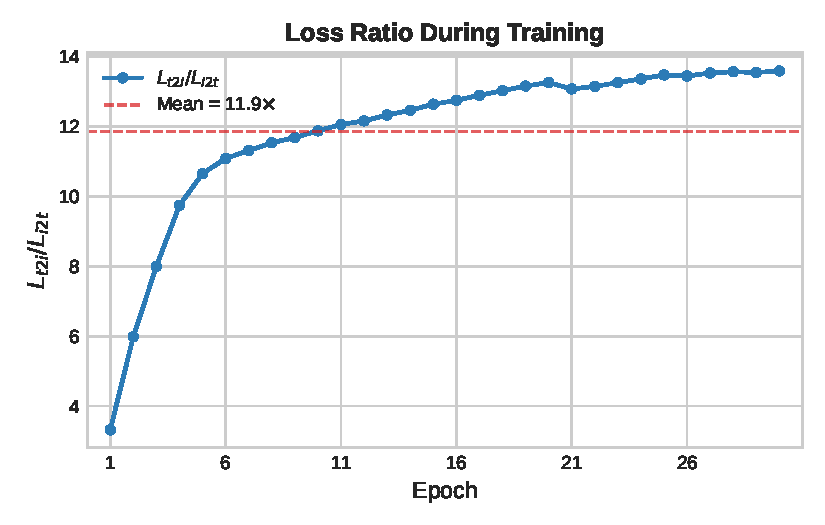
\includegraphics[width=0.72\textwidth]{figures/loss_ratio.pdf}
\caption{
\label{fig:loss_ratio}
Ratio of raw (unweighted) text-to-image loss to image-to-text loss $L_{t2i}/L_{i2t}$ during training with $\alpha{=}0.75$.
Despite the explicit optimization bias favoring t2i, the ratio increases from approximately 3.3$\times$ in the first epoch to over 13.5$\times$ by convergence, with a mean of $11.86\times$ (dashed line).
This growing gap demonstrates that the queue-induced asymmetry dominates the effect of loss reweighting.
}
\end{figure}

\subsection{Resource Constraints Naturally Lead to the Asymmetric Design}

The asymmetric queue is not an arbitrary design choice. Rather, it emerges naturally from our resource-constrained training setup: freezing the CLIP vision encoder keeps image and video embeddings perpetually fresh, while the evolving text encoder renders queued text embeddings stale. Under this setup, retaining only the image queue becomes the most natural solution.

\subsection{Stack LoRA for Efficient Domain Transfer}

The two-stage results (Tables~\ref{tab:video_results}, \ref{tab:flickr_results}) reveal a clear pattern: Stack LoRA achieves strong video retrieval (28.13~t2i~R@1 on MSVD) while converging faster than the full-parameter alternative (25 vs.\ 28 epochs). In contrast, simply continuing to fine-tune the full r=8 adapter without weight merging and re-stacking yields only 26.95~t2i~R@1---on par with the CLIP baseline and 1.18 points below Stack LoRA---indicating that the weight-merging and stacking strategy is essential for effective domain specialization.

Stack LoRA's smaller r=2 adapter, with its limited representational capacity, can only capture the most salient signal in the training data---and the most salient signal is precisely this image-to-video domain shift. The low-rank constraint forces the adapter to commit strongly to the target domain, yielding faster convergence (the optimizer searches a smaller space) and higher video retrieval (every trainable parameter is dedicated to the video shift). This specialization naturally shifts the text embedding distribution from the COCO-aligned space toward the video domain, which explains the observed Flickr degradation ($-$3.58) as a predictable consequence rather than a limitation.

Crucially, this pluggability is a natural property of LoRA-based adaptation. The COCO-aligned r=8 adapter and the MSR-VTT r=2 stack are separate low-rank matrices that can be loaded, swapped, or composed at inference time with negligible memory overhead. When the task is image retrieval, only the r=8 adapter is needed; when the domain shifts to video, the r=2 stack can be plugged in on top without discarding the original alignment. Since each adapter adds a fraction of the full model size (1.35M~parameters for r=8, 0.63M for r=2) and both fit comfortably on a single 8\,GB GPU, users can maintain multiple domain-specific adapters and deploy them as needed---a practical instantiation of the parameter-efficient philosophy.

\subsection{Extending to Multilingual Retrieval}

Our framework's reliance on BERT as the text encoder naturally extends to multilingual settings, since BERT provides multilingual variants (e.g., bert-base-multilingual-cased) with a shared tokenizer and embedding space across languages. To probe this capability, we train a multilingual BERT with identical hyperparameters on the same English COCO captions and evaluate zero-shot on Chinese Flickr30k, where Chinese captions are obtained by translating the original English captions using HY-MT1.5~\citep{hymt152025tencent}.

\begin{table}[h]
\centering
\caption{Zero-shot multilingual retrieval on Flickr30k. All models are trained on English COCO captions only.}
\label{tab:multilingual}
\begin{tabular}{lcc}
\toprule
Method & t2i R@1 & i2t R@1 \\
\midrule
BERT-uncased (EN, Ours) & 60.48 & 74.60 \\
Multilingual BERT (EN, Ours) & 57.08 & 69.00 \\
Multilingual BERT (ZH, Ours) & 27.22 & 39.20 \\
\bottomrule
\end{tabular}
\end{table}

Table~\ref{tab:multilingual} reports the multilingual results. The multilingual BERT achieves 57.08\% English t2i R@1, a 3.4-point degradation from BERT-uncased (60.48\%), attributable to the multilingual tokenizer's reduced sub-word efficiency for English text. More importantly, it attains 27.22\% t2i R@1 on Chinese---substantially above the 0.1\% random baseline and nearly half of its English performance---despite never having seen Chinese text during training. This demonstrates meaningful zero-shot cross-lingual transfer: the shared multilingual embedding space, when aligned to CLIP's visual representations through English-only contrastive learning, generalizes to non-English queries.

These results further illustrate the pluggability of our BERT-based framework. Because the LoRA adapter operates on BERT's internal representations rather than language-specific features, the same English-trained adapter applies to multilingual BERT without modification. In a video retrieval context, this means a multilingual BERT aligned to CLIP's visual space can retrieve videos using queries in multiple languages, and the Stack LoRA video-domain adapter transfers alongside the base model without requiring multilingual video training data.

\section{Limitations}

We acknowledge several limitations in this work. First, our video evaluation is limited to MSVD, which is a relatively small benchmark (1,970 videos; we use the standard 670-video test split). Larger and more diverse video retrieval benchmarks such as MSR-VTT 1K-A or ActivityNet would provide a more comprehensive assessment. The use of simple mean pooling for frame aggregation also limits our ability to capture temporal structure in videos.

Second, our models are trained exclusively on COCO train2017 captions (113k images, 567k captions) for Stage~1, a single dataset with limited domain diversity. While this allows us to demonstrate the effectiveness of our approach under tight compute constraints, training on a more diverse corpus would likely improve generalization.

Third, evaluation on Flickr30k is conducted on a 1K test set where R@K metrics may have higher variance than on larger benchmarks.

Fourth, the ablation experiments report single-run results without confidence intervals. Due to compute constraints, each configuration was evaluated once rather than with multiple random seeds, so the observed differences should be interpreted with caution.

Fifth, our multilingual evaluation is limited to Chinese on a single dataset (Flickr30k) using machine-translated rather than human-annotated captions. The translation quality of HY-MT1.5~\citep{hymt152025tencent} may introduce noise that underestimates the true cross-lingual transfer capability, and the evaluation on additional languages and video benchmarks remains for future work.

\section{Future Work}

Several directions are worth exploring beyond this work. First, the simple mean pooling of frame embeddings can be replaced with more sophisticated temporal aggregation methods, such as a lightweight Transformer over the frame embedding sequence or cross-modal attention between text queries and video frames \citep{gorti2022xpool}. This could better capture motion and event structure, particularly on longer videos.

Second, evaluating on larger and more diverse video benchmarks (e.g., MSR-VTT 1K-A, ActivityNet, DiDeMo) would provide a more thorough assessment of generalization. Extending the framework to support multilingual video retrieval, where queries in different languages retrieve from the same video pool, is a natural application of our BERT-based approach.

Third, exploring more aggressive parameter efficiency (e.g., prompt tuning \citep{huang2023vop} or sparse adapters \citep{cao2024acl}) could further reduce the adaptation cost, and applying Stack LoRA to other domain transfer scenarios (e.g., image$\to$medical, English$\to$multilingual) would test its generality.

\section{Conclusion}

We presented Eureka-from-CLIP, a framework for replacing CLIP's text encoder with a lightweight BERT adapter for zero-shot text-to-video retrieval under tight resource constraints. Through a two-stage approach --- first aligning BERT to CLIP's visual space on COCO images (Stage~1), then domain-adapting to video via Stack LoRA (Stage~2) --- we achieve competitive results on both benchmarks: 60.48\% t2i R@1 on Flickr30k image retrieval (surpassing CLIP's 57.90\%) and 28.13\% t2i R@1 on MSVD video retrieval (outperforming CLIP's 27.01\%), all with only 0.63--1.35M trainable parameters on a single 8\,GB GPU.

Our text-staleness-aware asymmetric queue design addresses the fundamental challenge of training only the text encoder with a contrastive queue: by masking stale text embeddings while retaining the fresh image queue, we prevent gradient contamination and maximize the benefit of abundant negatives. Stack LoRA demonstrates that freezing a pre-trained adapter and stacking a smaller one can efficiently transfer cross-modal alignment to new domains with minimal computational overhead.

Our approach provides a practical, generalizable recipe for substituting CLIP's text encoder with arbitrary BERT variants, enabling video, multilingual, and domain-specific retrieval applications without expensive retraining from scratch.

\section*{Acknowledgments}

The authors thank Jie Lei for guidance and helpful discussions throughout this project. This work was completed as a course project for Python Application Development Foundation at Zhejiang University of Technology.

\bigskip

\bibliographystyle{plainnat}
\begin{thebibliography}{99}

\bibitem[Radford et al.(2021)Radford, Kim, Hallacy, Ramesh, Goh, Agarwal, Sastry, Askell, Mishkin, Clark, Krueger, and Sutskever]{radford2021clip}
A.~Radford, J.~W.~Kim, C.~Hallacy, A.~Ramesh, G.~Goh, S.~Agarwal, G.~Sastry, A.~Askell, P.~Mishkin, J.~Clark, G.~Krueger, and I.~Sutskever.
\newblock Learning transferable visual models from natural language supervision.
\newblock In \textit{ICML}, 2021.

\bibitem[Devlin et al.(2019)Devlin, Chang, Lee, and Toutanova]{devlin2019bert}
J.~Devlin, M.-W.~Chang, K.~Lee, and K.~Toutanova.
\newblock BERT: Pre-training of deep bidirectional transformers for language understanding.
\newblock In \textit{NAACL-HLT}, 2019.

\bibitem[He et al.(2020)He, Fan, Wu, Xie, and Girshick]{he2020moco}
K.~He, H.~Fan, Y.~Wu, S.~Xie, and R.~Girshick.
\newblock Momentum contrast for unsupervised visual representation learning.
\newblock In \textit{CVPR}, 2020.

\bibitem[Hu et al.(2022)Hu, Shen, Wallis, Allen-Zhu, Li, Wang, Wang, and Chen]{hu2022lora}
E.~J.~Hu, Y.~Shen, P.~Wallis, Z.~Allen-Zhu, Y.~Li, S.~Wang, L.~Wang, and W.~Chen.
\newblock LoRA: Low-rank adaptation of large language models.
\newblock In \textit{ICLR}, 2022.

\bibitem[Chen et al.(2022)Chen, Liu, Zhang, Ye, Yang, and Wu]{chen2022altclip}
Z.~Chen, G.~Liu, B.-W.~Zhang, F.~Ye, Q.~Yang, and L.~Y.~Wu.
\newblock AltCLIP: Altering the language encoder in CLIP for extended language capabilities.
\newblock \textit{arXiv preprint arXiv:2211.06679}, 2022.

\bibitem[Yang et al.(2022)Yang, Pan, Lin, Men, Zhang, Zhou, and Zhou]{yang2022chinese}
A.~Yang, J.~Pan, J.~Lin, R.~Men, Y.~Zhang, J.~Zhou, and C.~Zhou.
\newblock Chinese CLIP: Contrastive vision-language pretraining in Chinese.
\newblock \textit{arXiv preprint arXiv:2211.01335}, 2022.

\bibitem[van den Oord et al.(2018)van den Oord, Li, and Vinyals]{oord2018representation}
A.~van den Oord, Y.~Li, and O.~Vinyals.
\newblock Representation learning with contrastive predictive coding.
\newblock \textit{arXiv preprint arXiv:1807.03748}, 2018.

\bibitem[Plummer et al.(2015)Plummer, Wang, Cervantes, Caicedo, Hockenmaier, and Lazebnik]{plummer2015flickr30k}
B.~A.~Plummer, L.~Wang, C.~M.~Cervantes, J.~C.~Caicedo, J.~Hockenmaier, and S.~Lazebnik.
\newblock Flickr30k entities: Collecting region-to-phrase correspondences for richer image-to-sentence models.
\newblock In \textit{ICCV}, 2015.

\bibitem[Lin et al.(2014)Lin, Maire, Belongie, Hays, Perona, Ramanan, Dollár, and Zitnick]{lin2014coco}
T.-Y.~Lin, M.~Maire, S.~Belongie, J.~Hays, P.~Perona, D.~Ramanan, P.~Dollár, and C.~L.~Zitnick.
\newblock Microsoft COCO: Common objects in context.
\newblock In \textit{ECCV}, 2014.

\bibitem[Conneau et al.(2020)Conneau, Khandelwal, Goyal, Chaudhary, Wenzek, Guzmán, Grave, Ott, Zettlemoyer, and Stoyanov]{conneau2020xlmr}
A.~Conneau, K.~Khandelwal, N.~Goyal, V.~Chaudhary, G.~Wenzek, F.~Guzmán, E.~Grave, M.~Ott, L.~Zettlemoyer, and V.~Stoyanov.
\newblock Unsupervised cross-lingual representation learning at scale.
\newblock In \textit{ACL}, 2020.

\bibitem[Zhai et al.(2022)Zhai, Wang, Mustafa, Steiner, Keysers, Kolesnikov, and Beyer]{zhai2022lit}
X.~Zhai, X.~Wang, B.~Mustafa, A.~Steiner, D.~Keysers, A.~Kolesnikov, and L.~Beyer.
\newblock LiT: Zero-shot transfer with locked-image text tuning.
\newblock In \textit{CVPR}, 2022.

\bibitem[Zhai et al.(2023)Zhai, Mustafa, Kolesnikov, and Beyer]{zhai2023sigmoid}
X.~Zhai, B.~Mustafa, A.~Kolesnikov, and L.~Beyer.
\newblock Sigmoid loss for language image pre-training.
\newblock In \textit{ICCV}, 2023.

\bibitem[Sharma et al.(2018)Sharma, Ding, and
  Soricut]{sharma2018conceptual}
P.~Sharma, N.~Ding, and R.~Soricut.
\newblock Conceptual captions: A cleaned, hypernymed, image alt-text dataset for
  automatic image captioning.
\newblock In \textit{ACL}, 2018.

\bibitem[Thomee et al.(2016)Thomee, Shamma, Friedland, Elizalde, Ni, Poland,
  Borth, and Li]{thomee2016yfcc100m}
B.~Thomee, D.~A.~Shamma, G.~Friedland, B.~Elizalde, K.~Ni, D.~Poland,
  D.~Borth, and L.-J.~Li.
\newblock YFCC100M: The new data in multimedia research.
\newblock \textit{Communications of the ACM}, 59(2):64--73, 2016.

\bibitem[Tencent Hunyuan Team(2025)]{hymt152025tencent}
Tencent Hunyuan Team.
\newblock HY-MT1.5 technical report.
\newblock \textit{arXiv preprint arXiv:2512.24092}, 2025.

\bibitem[Luo et al.(2022)Luo, Ji, Zhong, Chen, Lei, Duan, and Li]{luo2022clip4clip}
H.~Luo, L.~Ji, M.~Zhong, Y.~Chen, W.~Lei, N.~Duan, and T.~Li.
\newblock CLIP4Clip: An empirical study of CLIP for end to end video clip retrieval.
\newblock \textit{Neurocomputing}, 508:293--304, 2022.

\bibitem[Bain et al.(2021)Bain, Nagrani, Varol, and Zisserman]{bain2021frozen}
M.~Bain, A.~Nagrani, G.~Varol, and A.~Zisserman.
\newblock Frozen in time: A joint video and image encoder for end-to-end retrieval.
\newblock In \textit{ICCV}, 2021.

\bibitem[Lei et al.(2021)Lei, Li, Zhou, Gan, Berg, Bansal, and Liu]{lei2021clipbert}
J.~Lei, L.~Li, L.~Zhou, Z.~Gan, T.~L.~Berg, M.~Bansal, and J.~Liu.
\newblock Less is more: ClipBERT for video-and-language learning via sparse sampling.
\newblock In \textit{CVPR}, 2021.

\bibitem[Gorti et al.(2022)Gorti, Vouitsis, Ma, Golestan, Volkovs, Garg, and Yu]{gorti2022xpool}
S.~K.~Gorti, N.~Vouitsis, J.~Ma, K.~Golestan, M.~Volkovs, A.~Garg, and G.~Yu.
\newblock X-pool: Cross-modal language-video attention for text-video retrieval.
\newblock In \textit{CVPR}, 2022.

\bibitem[Huang et al.(2023)Huang, Gong, Pan, Jiang, Lv, Li, and Wang]{huang2023vop}
S.~Huang, B.~Gong, Y.~Pan, J.~Jiang, Y.~Lv, Y.~Li, and D.~Wang.
\newblock VoP: Text-video co-operative prompt tuning for cross-modal retrieval.
\newblock In \textit{CVPR}, 2023.

\bibitem[Cao et al.(2024)Cao, Tang, Huang, Jin, Zhang, Liu, Chen, Liang, Yuan, and Li]{cao2024acl}
M.~Cao, H.~Tang, J.~Huang, P.~Jin, C.~Zhang, R.~Liu, L.~Chen, X.~Liang, L.~Yuan, and G.~Li.
\newblock RAP: Efficient text-video retrieval with sparse-and-correlated adapter.
\newblock In \textit{ACL Findings}, 2024.

\bibitem[Liu et al.(2022)Liu, Xiong, Xu, Cao, and Jin]{liu2022ts2net}
Y.~Liu, P.~Xiong, L.~Xu, S.~Cao, and Q.~Jin.
\newblock TS2-Net: Token shift and selection transformer for text-video retrieval.
\newblock In \textit{ECCV}, 2022.

\bibitem[Chen and Dolan(2011)]{chen2011collecting}
D.~Chen and W.~Dolan.
\newblock Collecting highly parallel data for paraphrase evaluation.
\newblock In \textit{ACL}, 2011.

\end{thebibliography}

\section{Hyperparameter Selection}

We evaluate $\alpha \in \{0.25, 0.50, 0.75\}$. Although $\alpha{=}0.50$ already achieves comparable performance, $\alpha{=}0.75$ yields the highest t2i R@1 and is therefore adopted in the final model. Table~\ref{tab:hyperparams} summarizes the key hyperparameters used in our framework. All experiments use LoRA rank $r=8$ trained on COCO captions with seed 42.

\begin{table}[h]
\centering
\caption{Key hyperparameters. CLIP ViT-B/32 (OpenAI) baseline: t2i R@1~57.90\%, i2t R@1~76.90\%.}
\label{tab:hyperparams}
\begin{tabular}{lcc}
\toprule
Hyperparameter & Value & Description \\
\midrule
Batch size & 128 & Max for 8 GB VRAM \\
Learning rate & $3\times10^{-4}$ & AdamW, cosine decay \\
Weight decay & 0.01 & \\
Warmup steps & 34,536 & Linear warmup \\
Epochs & 30 & \\
\midrule
LoRA rank $r$ & 8 & \\
LoRA $\alpha$ & 16 & \\
LoRA dropout & 0.1 & \\
LoRA targets & Q, K, V, O & BERT linear layers \\
\midrule
Queue size & 49,152 & FIFO contrastive queue \\
t2i weight $\alpha$ & 0.75 & Eq.~\ref{eq:asymmetric_loss} \\
Temperature $\tau$ init & $1/0.07$ & Learnable $\tau=\exp(\gamma)$ \\
\midrule
AMP & true & Mixed precision \\
\bottomrule
\end{tabular}
\end{table}

\end{document}
